\documentclass[svgnames,11pt]{beamer}
\input{/home/tof/Documents/Cozy/latex-include/preambule_commun.tex}
\input{/home/tof/Documents/Cozy/latex-include/preambule_beamer.tex}
%\usepackage{pgfpages} \setbeameroption{show notes on second screen=left}
\author[]{Christophe Viroulaud}
\title{Orientation}
\date{\framebox{\textbf{}}}
%\logo{}
\institute{Seconde - SNT}

\begin{document}
\begin{frame}
\titlepage
\end{frame}
\section{Quel métier?}
\begin{frame}
    \frametitle{Quel métier?}
\begin{center}
    {\Large 85\% des emplois de 2030 n'existent pas encore.}
\end{center}
    
\note[item]{dans le numérique: intelligence artificielle, robotique, multivers\dots}
\note[item]{difficile d'avoir un choix très pointu dès la seconde: pentester}
\end{frame}
\begin{frame}
    \frametitle{}

    \begin{activite}
    \begin{enumerate}
        \item Se rendre sur le site \url{https://www.onisep.fr}
        \item Dans l'onglet \textbf{MÉTIER} parcourir la section \textbf{Des métiers selon mes goûts}
        \item Choisir trois thèmes préférentiels.
    \end{enumerate}
    \end{activite}

\end{frame}
\section{Après le bac}
\begin{frame}
    \frametitle{Après le bac}

    \begin{center}
    \centering
    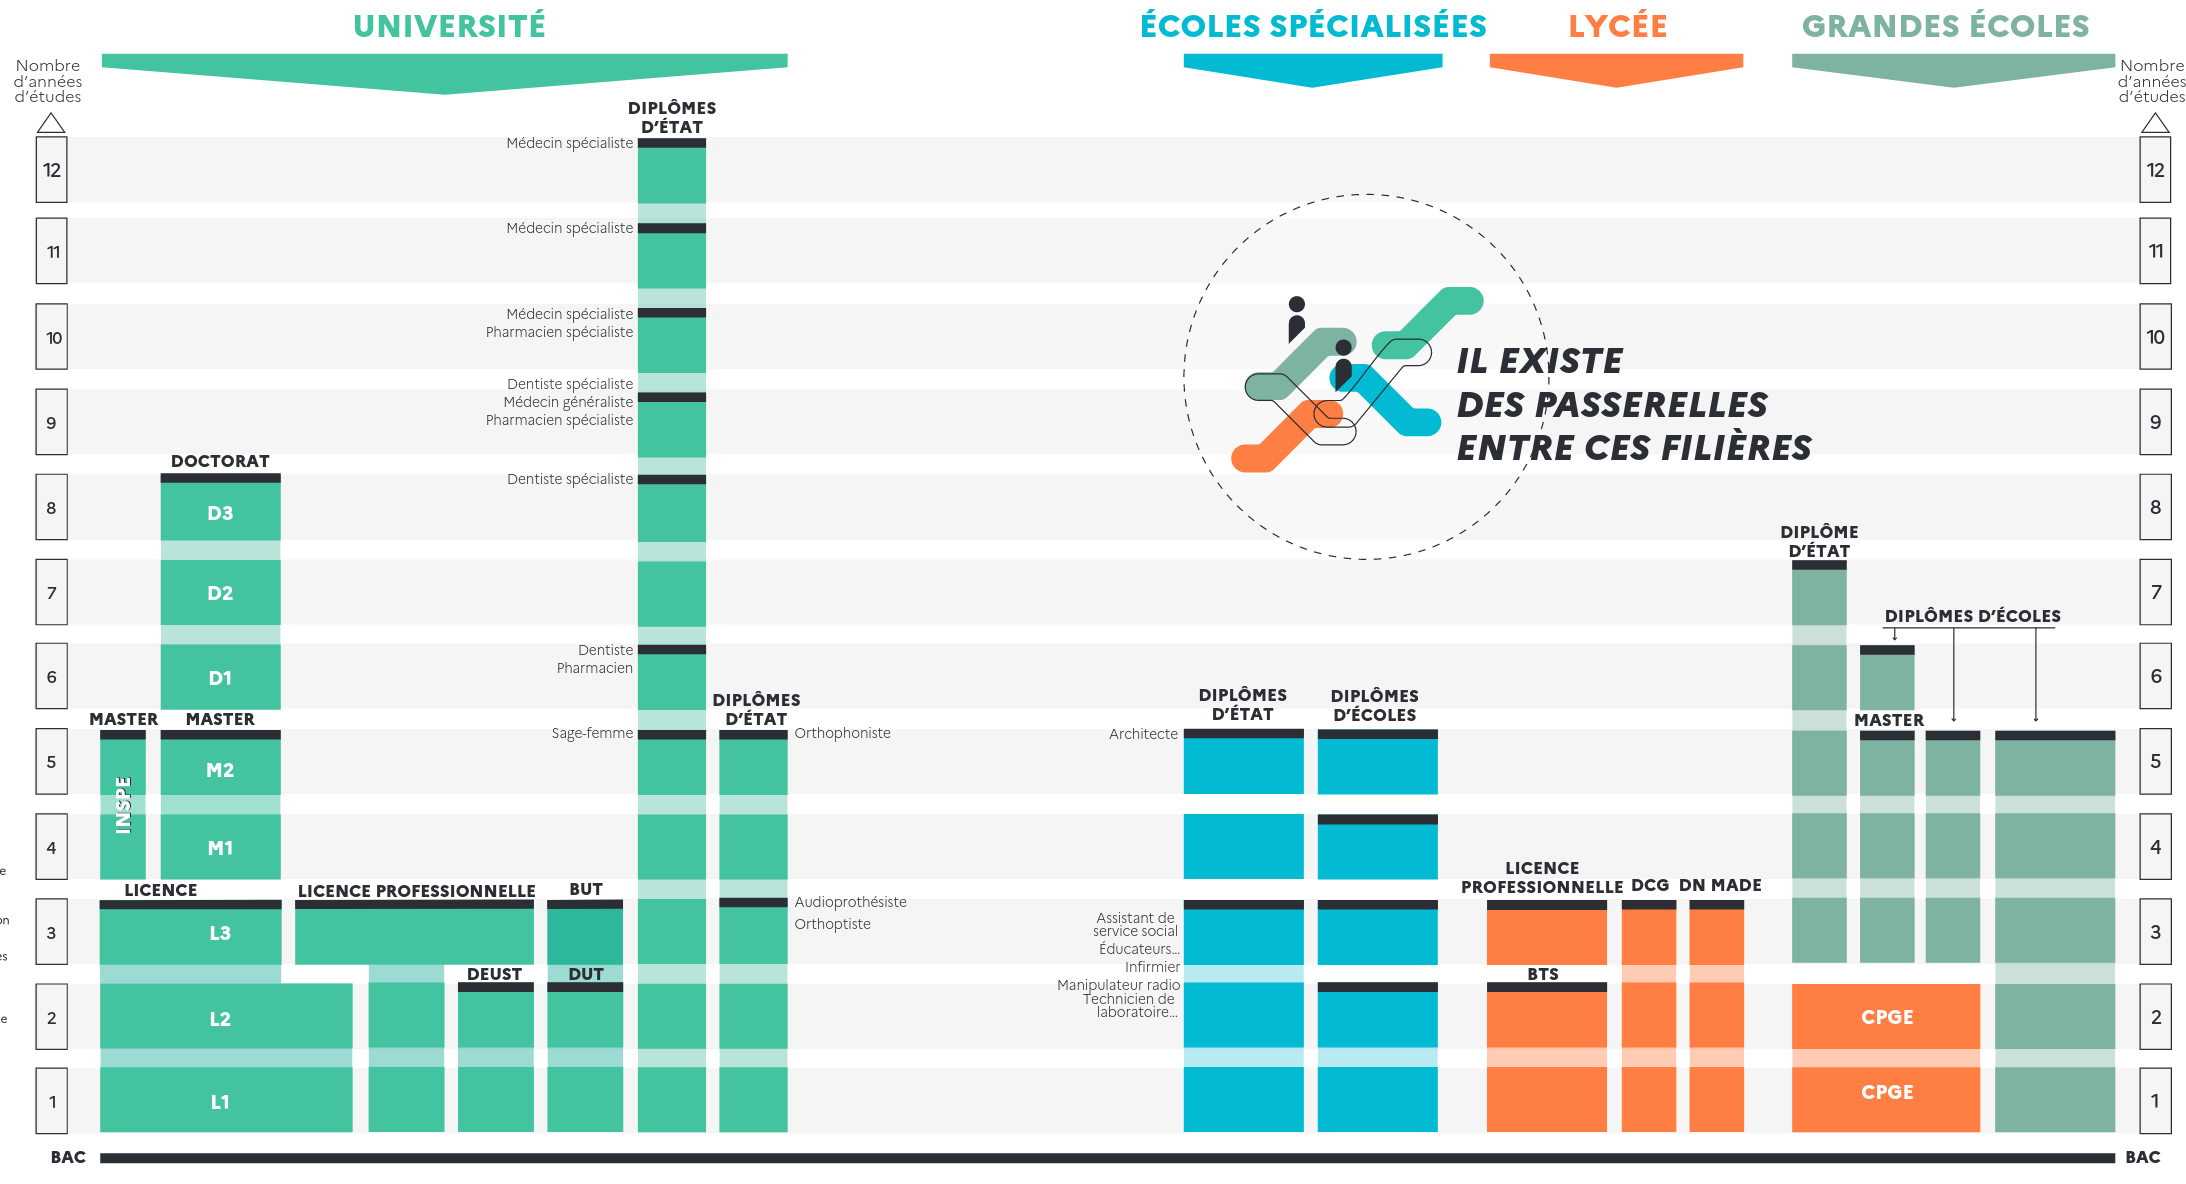
\includegraphics[width=12cm]{ressources/postbac.png}
    \end{center}

\end{frame}
\begin{frame}
    \frametitle{}

    \begin{activite}
    Déterminer la ou les voies correspondante(s) aux thèmes choisis précédemment. 
    \end{activite}

\end{frame}
\section{À partir de la Première}
\begin{frame}
    \frametitle{Voie générale}
\begin{itemize}
    \item Arts
    \item Biologie - Écologie
    \item Histoire - Géographie et Géopolitique
    \item Humanité, Littérature et Philosophie
    \item Mathématiques
    \item Numérique et Sciences Informatiques
    \item Sciences de la Vie et de la Terre
    \item Sciences de l'ingénieur
    \item Sciences Économiques et Sociales
    \item Physique - Chimie
    \item Langues et Littératures Étrangères
    \item Langues et Culture de l'Antiquité
    \item Éducation physique, Pratiques et Cultures Sportives
\end{itemize}

\end{frame}
\begin{frame}
    \frametitle{Voie technologique}

    \begin{itemize}
        \item STAV (Sciences et technologies de l'agronomie et du vivant)
        \item STD2A (Sciences et technologies du design et des arts appliqués)
        \item STI2D (Sciences et technologies de l'industrie et du développement durable)
        \item STL (Sciences et technologies de laboratoire)
        \item STMG (Sciences et technologies du management et de la gestion)
        \item ST2S (Sciences et technologies de la santé et du social)
        \item STHR (Sciences et technologies de l'hôtellerie et de la restauration)
        \item S2TMD (Sciences et techniques du théâtre, de la musique et de la danse)
    
    \end{itemize}

\end{frame}
\begin{frame}
    \frametitle{}

    \begin{activite}
    Pour chacune des voies, donner les spécialités qui sont enseignées au lycée Jay de Beaufort.
    \end{activite}

\end{frame}
\begin{frame}
    \frametitle{À Jay de Beaufort}

    \begin{itemize}
        \item Histoire - Géographie et Géopolitique
        \item Humanité, Littérature et Philosophie
        \item Mathématiques
        \item Numérique et Sciences Informatiques
        \item Sciences de la Vie et de la Terre
        \item Sciences Économiques et Sociales
        \item Physique - Chimie
        \item Langues et Littératures Étrangères
        \begin{itemize}
            \item Anglais
            \item Anglais monde contemporain
            \item Espagnol
        \end{itemize}
        \item Éducation physique, Pratiques et Cultures Sportives
    \end{itemize}

\end{frame}
\begin{frame}
    \frametitle{À Jay de Beaufort}

    \begin{itemize}
        \item STL (Sciences et technologies de laboratoire)
        \item ST2S (Sciences et technologies de la santé et du social)    
    \end{itemize}

\end{frame}
\begin{frame}
    \frametitle{}

    \begin{activite}
    En fonction des choix effectués précédemment, déterminer les spécialités générales ou filières technologiques correspondantes.
    \end{activite}

\end{frame}
\end{document}